\section{Sparse matrix multiplication} \label{sec:spmm}
Sparse matrix dense matrix multiplication (SpMM) leads to many random memory
accesses and its performance is usually limited by random memory throughput
of DRAM. We perform SpMM in semi-external memory (SEM)
to scale to a sparse matrix with billions of rows and columns. This strategy enables
nearly in-memory performance while achieving scalability in proportion
to the ratio of non-zero entries to rows or columns in a sparse matrix.

\subsection{Semi-external memory}
Our definition of semi-external memory for SpMM keeps the sparse matrix on
SSDs and the input dense matrix or some columns of the input dense matrix
in memory. We may keep the entire output matrix in memory if it is sufficiently
small to fit in memory, or stream the output matrix to SSDs or to the subsequent
computation to reduce memory consumption.

In some applications such as non-negative matrix factorization (Section
\ref{sec:spmm:apps}), even the input dense matrix cannot fit in memory. In this case,
we partition the input dense matrix vertically so that each partition has
complete columns of the original input dense matrix and can fit in memory.
For each vertical partition, we perform SpMM
in semi-external memory as before and stream the output matrix to SSDs.
%This approach requires $\lceil \frac{D}{M} \rceil$ passes over the sparse
%matrix, where $D$ is the storage size of the input dense matrix and $M$ is
%the memory size.

\subsection{Sparse matrix format}
To support efficient SpMM on graphs in semi-external memory, we design a new compact
sparse matrix format that increases CPU cache hits and reduces the amount of data
read from SSDs. A compact format is performance critical because in SEM-SpMM SSDs
are often the bottleneck.

Traditional sparse matrix formats such as compressed row storage (CSR) and
compressed column storage (CSC) are not designed for graphs. Graphs are sparse
and very large so the dense matrix involved in SpMM is too large to fit in CPU
cache. Furthermore, graphs usually have near-random vertex connection, which
leads to random access to rows in a large dense matrix in sparse matrix
multiplication. As such, these two formats cause
many CPU cache misses. In addition, these two formats also require a large
storage size. For a sparse matrix with billions of non-zero entries, we have to
use eight bytes to store row and column indices.

\begin{figure}
\centering
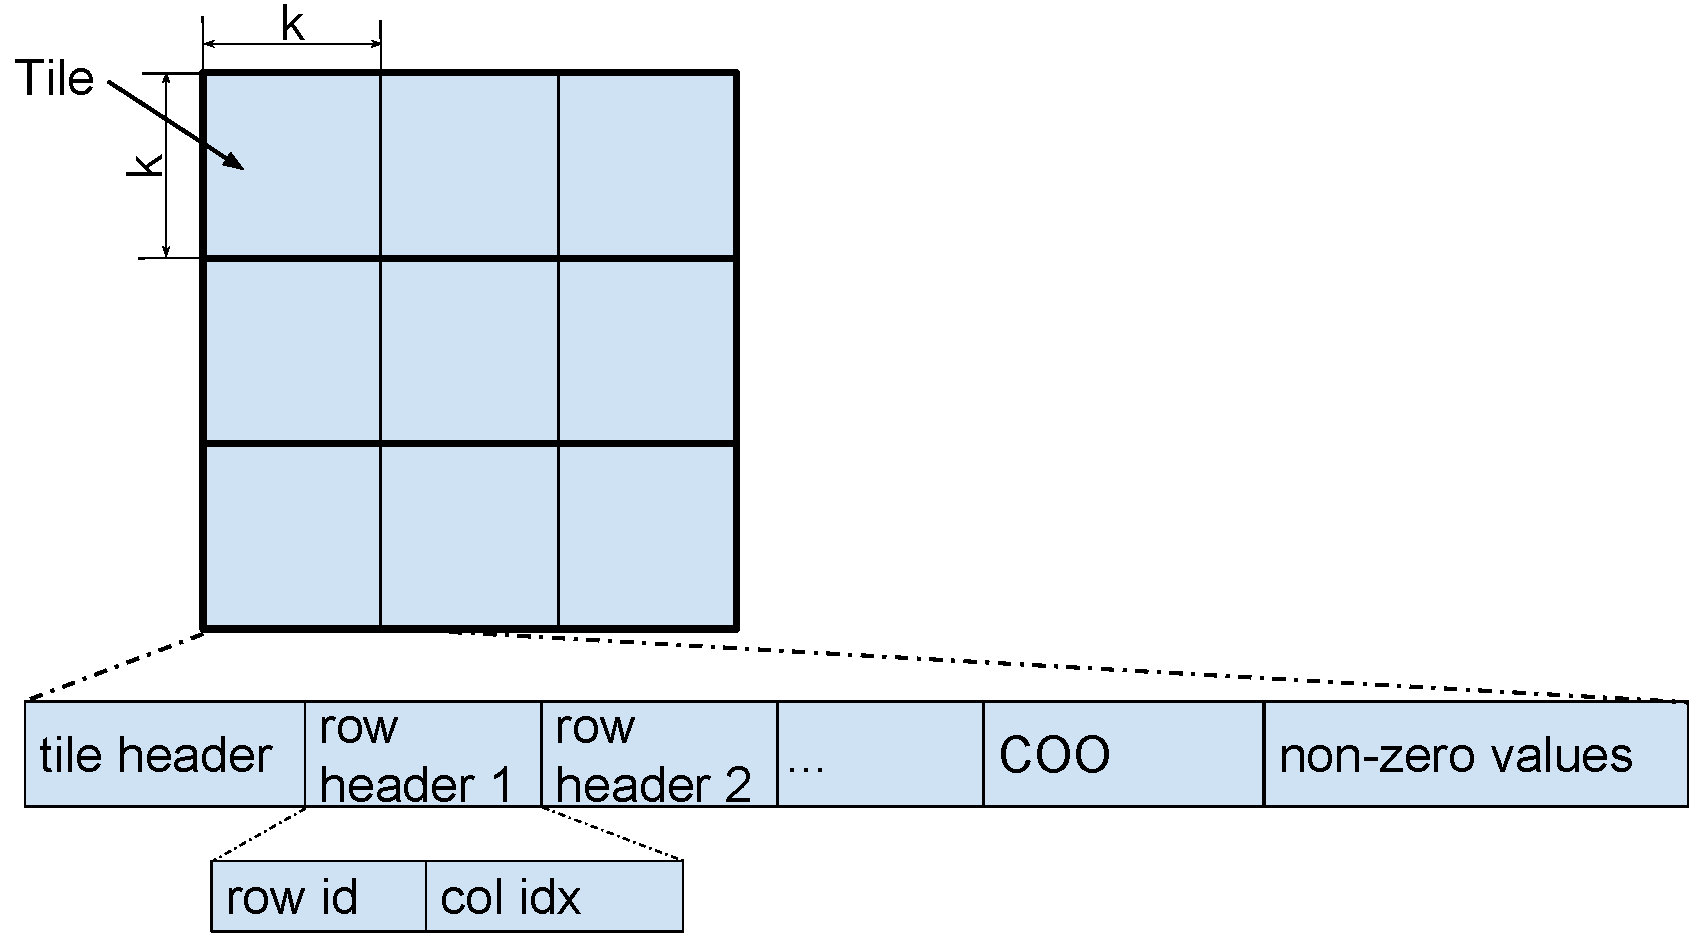
\includegraphics[scale=0.3]{SpMM_figs/sparse_mat.pdf}
\caption{The storage format of a sparse matrix. In this example, non-zero
entries of the sparse matrix are organized into 9 tiles. Tiles are stored in
the row-major order and a tile stores non-zero entries in SCSR+COO format.}
\label{sparse_mat}
\end{figure}

To increase CPU cache hits, we deploy cache blocking \cite{Im04} and store
non-zero entries of a sparse matrix in tiles, $t \times t$ submatrices (Figure
\ref{sparse_mat}).
When a tile is small, the rows from the input and output dense matrices
involved in multiplication with the tile are always kept in the CPU cache
during the computation. The optimal tile size should fill the CPU cache
with the rows from the dense matrices and is affected by the number of columns
of the dense matrices. To handle dense matrices with different numbers
of columns, we deploy both static cache blocking and dynamic cache blocking.
We generate sparse matrices with a relatively small tile size and
rely on the runtime system
to optimize for different numbers of columns (Section \ref{sec:exec}).
However, a small tile size potentially increases the storage size of a sparse
matrix. In semi-external memory, the dense matrices usually have
a very small number of columns in sparse matrix multiplication. Therefore, we
use the tile size of $16K \times 16K$ by default to balance the matrix storage
size and the adaptibility to different numbers of columns.

%\begin{figure}
%\centering
%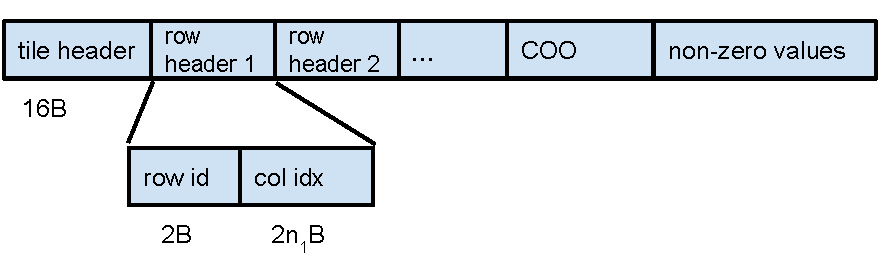
\includegraphics[scale=0.3]{SpMM_figs/tile_format.pdf}
%\caption{The storage format (SCSR + COO) of a tile in a sparse matrix.}
%\label{tile_format}
%\end{figure}

We use a very compact format to store non-zero entries and refer to this
format as SCSR (Super Compressed Row Storage) (Figure \ref{sparse_mat}).
In very sparse matrices many rows in a tile
do not have any non-zero entries. The CSR or CSC formats waste space because
they require an entry for each row/column in the row/column index. Doubly
compressed sparse column (DCSC) \cite{Buluc08} is proposed to avoid this problem.
However, even DCSC wastes space because it requires the storage of
pointers to columns and fails to reference to non-zero values with small
integers (e.g., two-byte integers). SCSR is designed to further shrink the storage
size of a tile.
Like DCSC, this format keeps data only for rows with non-zero entries in a tile.
Each non-empty row has a row header that only contains an identifier
to indicate the row number, followed by column indices. To determine the end
of a row, the most significant bit of the identifier is always set to 1, while
the most significant bit of a column index entry is always set to 0.
Owing to the small size of a tile, we use two bytes to store a row
number and a column index entry, which further reduces the storage size. As such,
each non-zero entry requires at most four bytes to indicate its location in
a matrix. Because the most significant bit is used to indicate the beginning
of a row, this format allows a maximum tile size of $32K \times 32K$.

SCSR is much more compact than DCSC \cite{Buluc08}. For a tile with $nnr$
non-empty rows and $nnz$ non-zero entries,
SCSR requires $2 \times nnr$ bytes for row ids, $2 \times nnz$ bytes for column
indices of non-zero entries and $c \times nnz$ bytes for non-zero values, where
$c$ is the number of
bytes for a non-zero value. As such, $S_{SCSR} = 2 \times nnr + (2 + c) \times nnz$.
In contrast, DCSC requires much more metadata for a tile
with $nnc$ non-empty columns and $nnz$ non-zero entries.
$S_{DCSC} = (2 + 2 + 4) \times nnc + (2 + c) \times nnz$. In a $t \times t$
tile, $nnr \le nnz \le nnr \times t$. On average, $nnr \approx nnc$ in most sparse
matrices. As such, for a binary sparse matrix, $0.4 \le S_{SCSR} / S_{DCSC} < 1$.
SCSR saves more space in a sparse matrix with larger $nnr / nnz$. Figure
\ref{fig:storage} shows that SCSR uses 45\%-70\% of the storage size used by DCSC
for large real-world graphs (Table \ref{graphs}).

\begin{figure}
	\begin{center}
		\footnotesize
		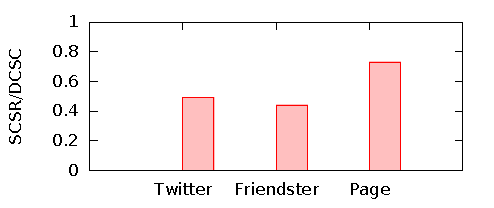
\includegraphics[scale=1]{SpMM_figs/storage.pdf}
		\caption{The ratio of the storage size required by SCSR and DCSC
			\cite{Buluc08} format for real-world graphs. SCSR is much more
		compact than DCSC for graphs.}
		\label{fig:storage}
	\end{center}
\end{figure}

Inside each cache tile of the SCSR, we use the coordinate format (COO) for
the rows that have only a single non-zero entry. For the adjacency matrices of
real-world graphs, many rows in a cache tile have only one non-zero entry,
owing to the sparsity of the graphs and nearly random vertex connection.
Iterating over single-entry rows in the SCSR format requires to test
the end of a row for every non-zero entry, which leads to many conditional jumps.
In contrast, COO is more suitable for storing these
single-entry rows. It does not increase the storage size but significantly
reduces the number of conditional jump instructions. As a result, we combine
SCSR with COO and store non-zero entries in the COO format behind the row headers
of SCSR (Figure \ref{sparse_mat}).

%We organize tiles in a sparse matrix in tile rows and maintain a matrix index
%for them. Each entry of the index stores the location of a tile row on SSDs
%to facilitate random access
%to tile rows. This is useful for parallelizing sparse matrix multiplication.
%Because a tile contains thousands of rows, the matrix index requires a very
%small storage size even for a billion-node graph. We keep the entire index
%in memory during sparse matrix multiplication.

\subsection{Dense matrices}
In many applications, the dense matrices in SpMM are tall and skinny with
millions or even billions of rows and a small number of columns.
The number of columns is determined by applications. Because many real-world graphs
are very large and sparse, the dense matrices may be too large to fit in memory.
Thus, for the general case of SpMM, we split the dense matrices into vertical
partitions of the memory size. To increase data locality in SpMM, the elements
in each vertical partition are stored in row-major order (Figure \ref{dense_mat}
(a)). When performing SpMM in semi-external memory, we load the input dense
matrix or one of its vertical partitions to memory if it is not in memory yet.

For a non-uniform memory architecture (NUMA), we partition the input dense matrix
or one of its vertical partitions horizontally and store horizontal partitions
evenly across NUMA nodes (Figure \ref{dense_mat} (b)). The NUMA architecture
is prevalent in today's multi-processor servers, where each processor connects
to its own memory banks. Therefore, keeping partitions evenly across all NUMA
nodes helps to fully utilize the bandwidth of memory and inter-processor links.
We assign multiple contiguous rows in a row interval with $2^i$ rows to
a NUMA node. The row interval size is multiple of the tile size of
a sparse matrix so that multiplication on a tile only needs to access rows
from a single row interval.

\begin{figure}
\centering
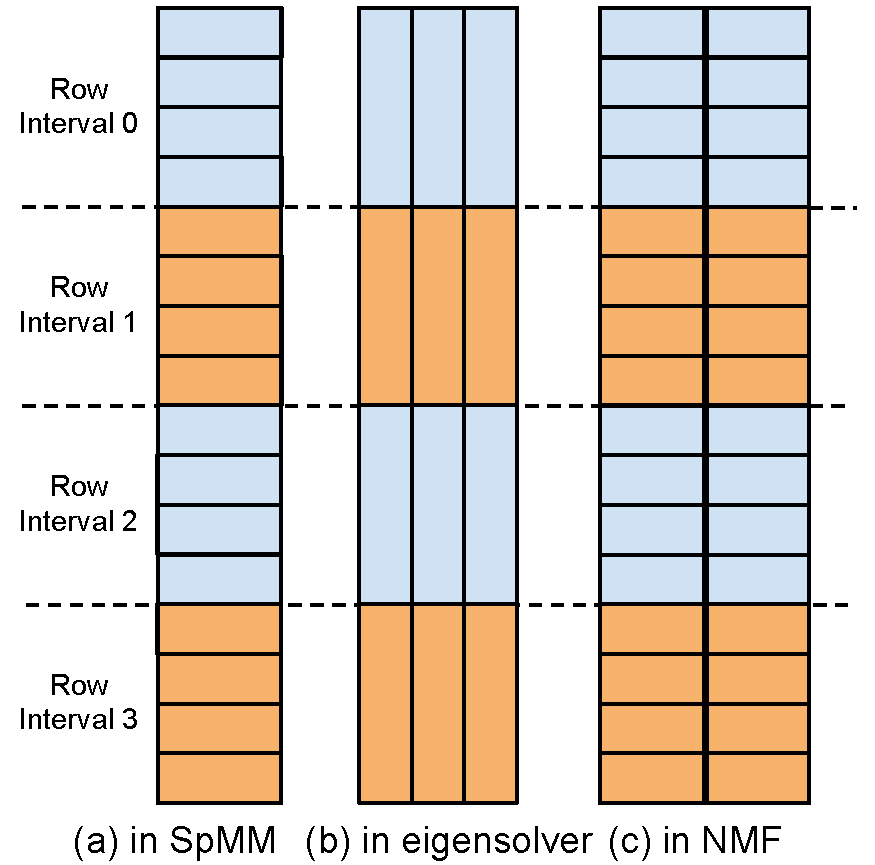
\includegraphics[scale=0.4]{SpMM_figs/dense_matrix.pdf}
\caption{The format of the dense matrices in SpMM. It is first partitioned
vertically so that each vertical partition can fit in memory. A vertical
partition stores data in row-major order. When a vertical partition is loaded
to NUMA memory, it is partitioned horizontally into many row intervals and
is stored across NUMA nodes.}
\label{dense_mat}
\end{figure}

\subsection{Parallel Execution} \label{sec:exec}
This section describes parallel execution of sparse matrix multiplication
in semi-external memory. Memory is precious resource in this computation model
because memory should be used to keep more columns in the input dense matrix
to reduce I/O from SSDs (as discussed in Section \ref{sec:spmm:mem}).
As such, we deploy only computation optimizations with a small memory footprint.
Algorithm \ref{alg:spmm} and Figure \ref{spmm_exec} illustrate the execution of
sparse matrix multiplication in semi-external memory.
%and the power-law distribution of non-zero entries in each row of a sparse
%matrix.

\begin{figure}
\centering
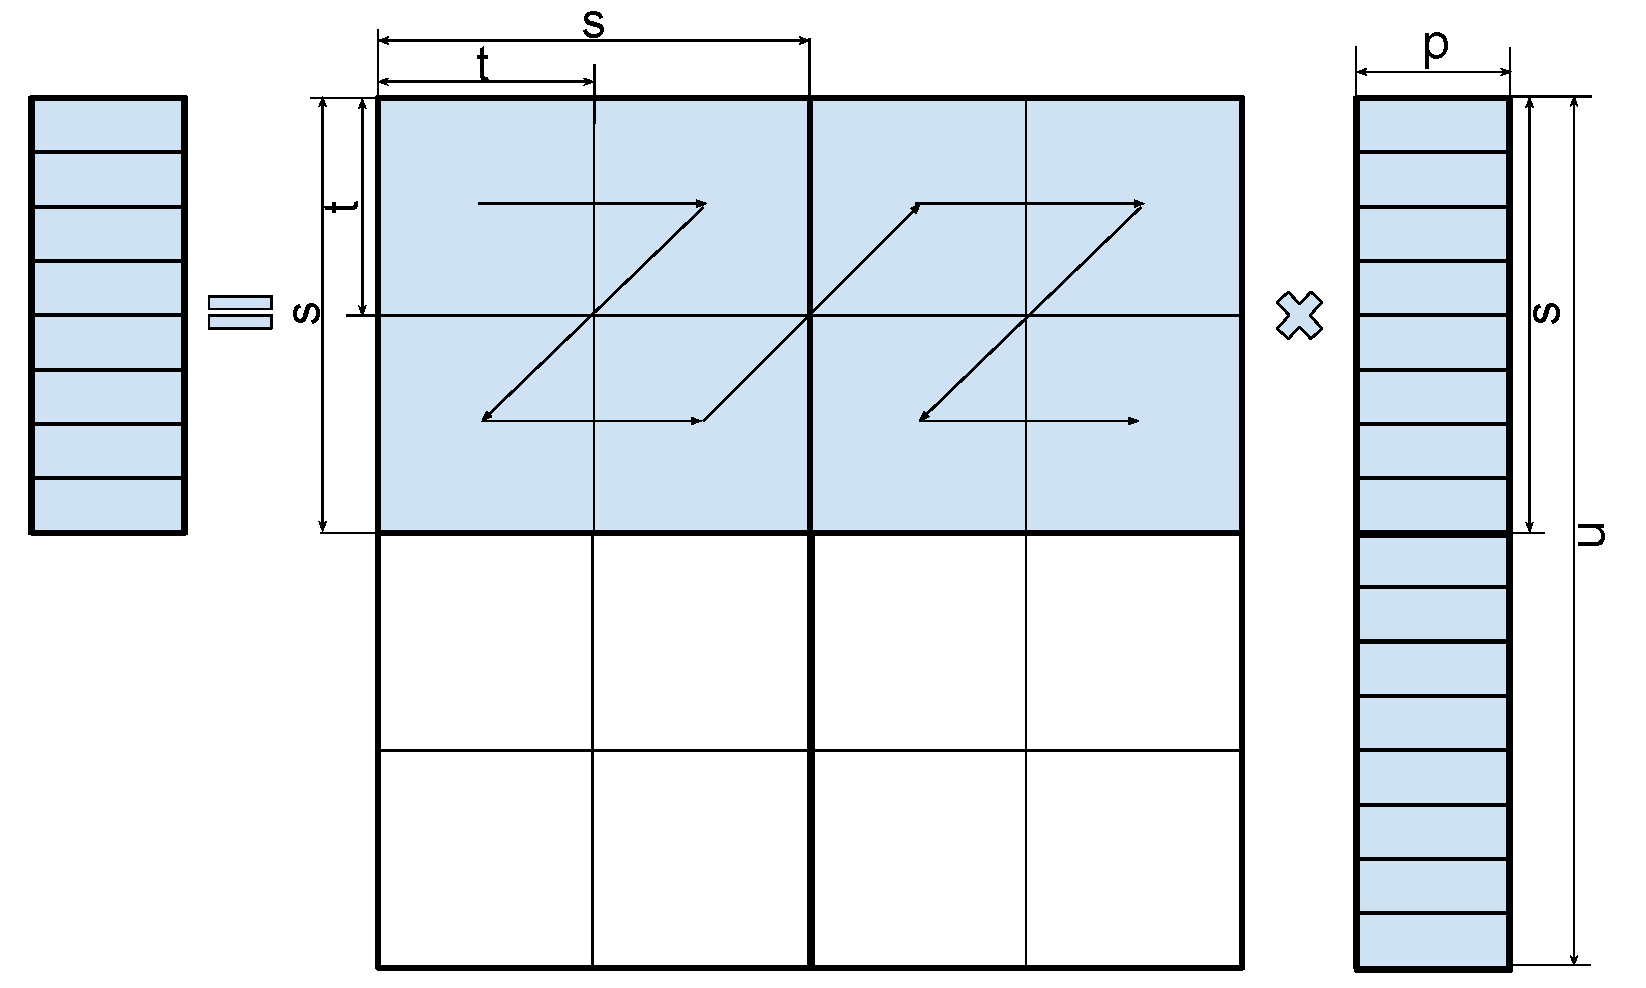
\includegraphics[scale=0.3]{SpMM_figs/SpMM_exec.pdf}
\caption{The execution of multiplication on tiles in a sparse matrix and
	the input dense matrix in a single thread. A thread reads $\frac{s}{t}$
	tile rows and multiplies them with the input dense matrix
	($s = \frac{CPU\_cache}{2 \times p}$). The arrows indicate the order
of multiplication on tiles with the input dense matrix.}
\label{spmm_exec}
\end{figure}

Semi-external memory favors horizontal partitioning on a sparse matrix
for parallelization because this partitioning scheme minimizes writes to SSDs
and remote memory with small memory consumption. Horizontal partitioning
requires only one thread to allocate local memory buffers for computation on
a tile row. All intermediate computation results on tiles are merged into
the local memory buffers. As such, we write the output matrix at most once
to SSDs and there are no remote memory writes.
In contrast, both vertical partitioning and 2D partitioning require each
thread to maintain a local memory buffer for the same tile rows in order
to reduce writes to SSDs and remote memory, which increases memory consumption.

\begin{algorithm}
	\algblock{ParFor}{EndParFor}
	% customising the new block
	\algnewcommand\algorithmicparfor{\textbf{parfor}}
	\algnewcommand\algorithmicpardo{\textbf{do}}
	\algnewcommand\algorithmicendparfor{\textbf{end\ parfor}}
	\algrenewtext{ParFor}[1]{\algorithmicparfor\ #1\ \algorithmicpardo}
	\algrenewtext{EndParFor}{\algorithmicendparfor}

	\caption{Parallel execution of sparse matrix dense matrix multiplication.}
	\label{alg:spmm}
	\begin{algorithmic}[1]
		\Procedure{SparseMatrixMultiply}{$spm$, $inM$}
		\Statex \textbf{Input}: $spm$, a $n \times n$ sparse matrix on SSDs
		\Statex \textbf{Input}: $inM$, a $n \times p$ dense matrix in memory
		\Statex \textbf{Output}: $outM$, a $n \times p$ dense matrix on SSDs
		\State $\vec{trQ} \gets get\_tile\_row\_ids(spm)$
		\State $outM \gets zeros\_SSD(n, p)$
		\ParFor{$thread \in \vec{threads}$}
		\State $ProcessTileRows(spm, \vec{trQ}, inM, outM)$
		\EndParFor
		\EndProcedure

		\State

		\Procedure{ProcessTileRows}{$spm$, $\vec{trQ}$, $inM$, $outM$}
		\Statex \textbf{Input}: $spm$, a $n \times n$ sparse matrix on SSDs
		\Statex \textbf{Input}: $\vec{trQ}$, a queue that contains all tile row ids
		\Statex \textbf{Input}: $inM$, a $n \times p$ input dense matrix in memory
		\Statex \textbf{In-Out}: $outM$, a $n \times p$ output dense matrix on SSDs
		\State $t \gets get\_tile\_size(spm)$
		\State $numTRs \gets \frac{CPU\_cache\_size}{2 \times p \times t}$
		\While{$|\vec{trQ}| > 0$}
		\If {$|\vec{trQ}| <= \#threads$}
		\State $numTRs \gets 1$
		\EndIf
		\State $\vec{ids} \gets get\_tile\_rows(\vec{trQ}, numTRs)$
		\State $trs \gets read\_tilerow\_async(spm, \vec{ids})$
		\State $res \gets MulTRows(trs, inM)$ when $trs$ is ready
		\State $write\_rows\_async(outM, res)$
		\EndWhile
		\EndProcedure

		\State

		\Procedure{MulTRows}{$trs$, $inM$}
		\Statex \textbf{Input}: $trs$, a $s \times n$ submatrix in the sparse matrix
		\Statex \textbf{Input}: $inM$, $n \times p$ dense matrix
		\Statex \textbf{Output}: $outBuf$, a $s \times p$ dense matrix
		\State $outBuf \gets zeros(s, p)$
		\State $t \gets get\_tile\_size(trs)$
		\For{$k=0; k < \frac{n}{t}; k = k + \frac{s}{t}$}
		\For{$i=0; i < \frac{s}{t}; i = i + 1$}
		\For{$j = 0; j < \frac{s}{t}; j = j + 1$}
		\State $tile \gets trs[i, k + j]$
		\State $lInMat \gets$ rows from $inM$ for $tile$
		\State $lOutMat \gets$ rows from $outBuf$ for $tile$
		\State $lOutMat += tile * lInMat$
		\EndFor
		\EndFor
		\EndFor
		\EndProcedure
	\end{algorithmic}
\end{algorithm}

We deploy a fine-grain dynamic load balancing scheme for parallel computation
with a global task queue \textit{trQ} (in Algorithm \ref{alg:spmm}). Each thread
gets one computation task (tile rows) at a time from \textit{trQ} with
\textit{get\_tile\_rows} and perform computation (\textit{MulTRows}).
At the beginning, a thread gets larger computation tasks that contains multiple
tile rows; as the computation approaches completion, a thread gets smaller
tasks that contain only one tile row. This design reduces concurrent access to
the global data structure while realizing good load balancing.

We further use the global task queue \textit{trQ} to help merge writes to
the output matrix on SSDs. Large writes ensure sustainable write throughput to
SSDs and increase their duration \cite{sfs}. To assist in I/O merging, we use
\textit{get\_tile\_rows()} to control a global execution
order that ensures that all threads are processing contiguous tile rows and
the results from the tile rows are located closely on SSDs. Given this execution
order, we write computation results from \textit{MulTRows} to SSDs
asynchronously with \textit{write\_rows\_async()}, which postpones writes,
merges writes from different threads and writes them to SSDs with a single I/O.

\textit{MulTRows} in Algorithm \ref{alg:spmm} processes tile rows that have
been read to memory. To better utilize the CPU cache, we reorganize $t \times t$
tiles from multiple contiguous tile rows into $s \times s$ blocks, where
$s = \frac{CPU\_cache}{2 \times p}$ (Figure \ref{spmm_exec}). We process all
tiles in a $s \times s$ block before moving to the next block. The tile size
of a sparse matrix is relatively small. As such, this execution order helps to
reuse data in the CPU cache from the computation on the previous tile.
\textit{MulTRows} also maintains
a local memory buffer $outBuf$ to store the computation results,
which minimizes remote memory access. Once the computation in \textit{MulTRows}
is complete, $outBuf$ contains complete results.

In spite of nearly random edge connection in a real-world graph, we explore
regularity in multiplying a tile with a partition of a row-major dense matrix.
In this case we multiply a non-zero entry from a tile with all elements in
a row of the input dense matrix and add the results to the corresponding row
of the output dense matrix.
We perform these operations with vector CPU instructions, such as
AVX \cite{avx} to enable more efficient memory access and computation.
The current implementation relies on GCC's auto-vectorization
to translate the C code to vector CPU instructions by predefining the matrix
width in the code.

\subsection{I/O optimizations}
Semi-external memory sparse matrix multiplication streams a sparse matrix from
SSDs, which results in sequential I/O. This I/O access pattern does not generate
any cache hits in the Linux page cache when the sparse matrix size is larger
than main memory. As such, we access a sparse matrix on SSDs with direct I/O.
For accessing data in fast SSDs sequentially, the overhead of operating systems
such as thread context switch and memory allocation becomes noticeable.
We tackle these obstacles to maximize I/O throughput.

We issue asynchronous I/O and poll for I/O to avoid thread
context switches because the latency of a context switch can undermine
the sequential I/O throughput of a high-speed SSD array. When a thread issues
an I/O request and waits for I/O completion, the operating system switches
the thread
out; the operating system reschedules the thread for execution once I/O is
complete. However, there is latency for thread rescheduling and the latency
from frequent rescheduling can cause noticeable performance degradation
on a high-speed SSD array. As such, we use I/O polling to avoid a thread from
being switched out after the thread completes all computation available to it.

When accessing a sparse matrix or a dense matrix from SSDs, we maintain a set of
memory buffers for I/O access to reduce the overhead of memory allocation.
We use large I/O to access matrices on SSDs to increase I/O throughput.
Large memory allocation is expensive because the operating
system usually allocates a large memory buffer with \textit{mmap()} and
populates the buffer with physical pages when it is used. Therefore, we keep
a set of memory buffers allocated previously and reuse them for new I/O requests.
For accessing a sparse matrix, tile rows usually have different sizes, so we resize
a previously allocated memory buffer if it is too small for a new I/O request.

\subsection{The impact of the memory size on I/O}
\label{sec:spmm:mem}
More memory reduces I/O in semi-external memory.
The minimum memory requirement for semi-external memory sparse matrix
multiplication is $n c + t \epsilon$, where $n$ is the number of rows
of the input dense matrix, $c$ is the element size in bytes,
$t$ is the number of threads processing the sparse matrix
and $\epsilon$ is the buffer size for the sparse matrix and the output
dense matrix. When a machine does not have sufficient memory to keep the entire
input dense matrix in memory, we need multiple passes on the sparse matrix to
complete the computation. Reducing memory consumption is essential
to achieve performance in semi-external memory. By keeping more columns of
the input dense matrix in memory, we reduce the number of I/O passes.

Although we can use some memory to cache part of the sparse matrix,
keeping more columns of the input dense matrix in memory saves more I/O than
using the same amount of memory to cache the sparse matrix. Assume the input
dense matrix has $n$ rows and $p$ columns. Again, $c$ is the element size
in bytes. The storage size of the sparse
matrix is $E$ bytes and the memory size is $M$ bytes. We further assume
we use $M'$ bytes to keep some columns of the dense matrices in memory
($M' < M$, ${n c p} \mod {M'} \equiv 0$)
and the remaining memory ($M - M'$) to cache the sparse matrix.
The amount of data in the sparse matrix read from SSDs is
\begin{equation*}
IO_{in} = \frac{n c p}{M'} [E - (M - M')]
\end{equation*}
Because $E > M$ in semi-external memory, we minimize $IO_{in}$ by maximizing $M'$.
Therefore, using memory for the input dense matrix always results in a smaller
amount of I/O than using memory for caching the sparse matrix.

As the number of columns in memory from the input dense matrix increases,
the bottleneck of the system
may switch. When we keep only one column of the input dense matrix in memory,
the system is usually I/O bound; when we keep more columns of the dense matrix
in memory, the system will become CPU bound and the I/O complexity does not
affect its performance.
%and the additional memory does not improve
%the performance of sparse matrix multiplication further.

%Our strategy results in the minimum amount of data written to SSDs. When the output
%dense matrix cannot fit in memory, the maximum write is $N k$ for a square
%sparse matrix.
%In other words, the output matrix only needs to be written to SSDs at most once.
%The additional memory in the system can be used to buffer part of the output
%dense matrix to reduce the amount of data written to SSDs. Streaming the output
%matrix directly to the subsequent matrix computation can also reduce data written
%to SSDs.

\subsection{I/O complexity}
The semi-external memory (SEM) solution for sparse matrix multiplication leads
to no more I/O than the external-memory (EM) solution for many real-world graphs.
The EM solution has both the sparse matrix and the input dense matrix on SSDs,
and only loads part of the matrices during computation. Writing data to SSDs
causes SSD wearout. The SEM solution minimizes writes to SSDs. To minimize writes,
the EM solution scans the sparse matrix once but reads the input dense matrix
multiple times.

When a machine has sufficient memory to keep the entire input dense matrix
in memory, the SEM solution only needs to read the sparse matrix and the input
dense matrix once and write the output dense matrix once. This is
the minimum amount of I/O.

When a machine has insufficient memory to keep the input dense matrix, the SEM
solution still leads to less I/O than the EM solution when $E < n c p t$ if we
minimize writes to SSDs.
In this analysis, we assume a square sparse matrix. The same analysis applies
to a rectangular sparse matrix as well.
In this case, the SEM solution scans the sparse matrix multiple times.
\begin{equation*}
read_{SEM} = \frac{n c p}{M} E + n c p
\end{equation*}
Due to near random vertex connection in real-world graphs, the EM solution needs to
read the entire input dense matrix each time. In the parallel setting,
the EM solution requires each thread to keep local memory buffers for portions
of the input and output dense matrices. Assume the EM solution keeps $j$ rows
from the input dense matrix and $i$ rows from the output dense matrix in memory
in each thread.
\begin{equation*}
(i c p + j c p) t = M \implies i < \frac{M}{c p t}
\end{equation*}
\begin{equation*}
read_{EM} = \frac{n}{i} n c p + E \implies  read_{EM} > \frac{n^2 c^2 p^2 t}{M} + E
\end{equation*}
When $n c p < E < n c p t$, $read_{EM} > read_{SEM}$.
When $E \leq n c p$, $read_{EM} > read_{SEM}$ for any $t \geq 2$.

As such, the SEM solution in practice causes less I/O in many natural graphs.
For the natural graphs that we have seen, such as Twitter \cite{twitter},
the Page graph \cite{web_graph} and Friendster \cite{friendster}, the number
of edges is of $10-100 \times$ the number of vertices. Essentially,
natural graphs have sparse edge matrices. We target multi-core machines with
10s to 100s of threads. For most of our applications, $p$ is of size 1-30.
For very small $p$, the SEM solution can keep the entire input dense matrix
in memory and leads to the minimum I/O. For a relatively larger $p$, $E < n c p t$
holds for most of natural graphs when the graphs are processed in a large
parallel machine. Therefore, the SEM solution usually performs less I/O than EM.

\section{Applications} \label{sec:spmm:apps}
We apply sparse matrix multiplication to three important applications widely
used in data mining and machine learning: PageRank \cite{pagerank},
eigensolver \cite{anasazi} and non-negative matrix factorization \cite{nmf}.
Each application demonstrates a different strategy of using memory for sparse
matrix multiplication.

\subsection{PageRank} \label{sec:pagerank}
PageRank is an algorithm to rank the Web pages by using hyperlinks between Web
pages. It was first used by Google and is identified as one of the top 10 data
mining algorithms \cite{top10}. PageRank is a representative of a set of graph
algorithms that can be expressed with sparse matrix multiplication or generalized
sparse matrix multiplication. Other important examples are label propagation
\cite{label_prop} and belief propagation \cite{Yedidia03}. The algorithm runs
iteratively and its update rule for each Web pages in an iteration is
\begin{equation*}
PR(u) = \frac{1-d}{N} + d \sum\limits_{v \in B(u)} \frac{PR(v)}{L(v)}
\end{equation*}
where $B(u)$ denotes the neighbor list of vertex $u$ and $L(v)$ denotes
the out-degree of vertex $v$. %We implement the PageRank algorithm with sparse
%matrix multiplication (Figure \ref{code:pagerank}).


%\begin{figure}
%\centering
%%\begin{minted}[mathescape, fontsize=\scriptsize,]{r}
%\begin{lstlisting}
%while (L1 >= epsilon && niters < max.niters) {
%	pr2 <- d/N+(1-d)*(A %*% (pr1/out.deg))
%	L1 <- sum(abs(pr1-pr2))
%	pr1 <- pr2
%	niters <- niters + 1
%}
%\end{lstlisting}
%%\end{minted}
%\caption{The implementation of PageRank \cite{pagerank} with SpMM.}
%\label{code:pagerank}
%\end{figure}

%Based on the memory size, we can place different data in memory to reduce I/O.
%When the memory can only fit a single vector, each iteration needs
%to write a vector to SSDs and read two vectors (the result from
%the previous iteration and the degree vector) and the sparse matrix
%from SSDs. When the memory can fit two vectors, the output vector can be kept
%in memory, so each iteration needs to read the sparse matrix and the degree vector
%and does not write any data to SSDs. As more memory can be used, we can
%further keep the degree vector and even cache part of the sparse matrix.

\subsection{Eigensolver}
An eigensolver is another commonly used application that requires sparse matrix
multiplication. Many algorithms \cite{Lanczos, IRLM, krylovschur} and frameworks
\cite{arpack, anasazi, slepc} have been developed to solve a large eigenvalue
problem.

We take advantage of the Anasazi eigensolver framework \cite{anasazi} and
replace its original matrix operations with our SEM sparse
matrix multiplication and external-memory dense matrix operations. To compute
eigenvalues of a $n \times n$ matrix, many eigenvalue algorithms for a large
sparse matrix require to construct a vector subspace with a sequence of
sparse matrix multiplications and each vector in the subspace has the length of $n$.
Due to the sparsity of real-world graphs, the vector subspace is large and we keep
vectors in the subspace on SSDs. In addition to sparse matrix
multiplication, eigensolvers perform some dense matrix operations on the subspace.
For example, eigensolvers need to orthogonalize the vectors in the subspace with
dense matrix multiplication. The Anasazi eigensolvers have block extension to
update multiple vectors in the subspace simultaneously, which results in sparse matrix dense
matrix multiplication. The most efficient Anasazi eigensolver on sparse graphs
is the KrylovSchur eigensolver \cite{krylovschur}, which updates a small number
of vectors (1-4) in the subspace simultaneously. Zheng et al.
\cite{flasheigen} provides the details of extending the Anasazi eigensolver
with external-memory matrix operations.

%The choice of data placement for an eigensolver is a little different from
%PageRank. If a machine has a small amount of memory, the memory should be
%used to keep the input dense matrix. If a machine has more memory, we should
%use it to buffer the output dense matrix. The dense matrices involved in
%sparse matrix multiplication have a small number of columns in
%the KrylovSchur eigensolver and usually can fit in memory. 
%Additional memory should be used to buffer the vectors in the subspace
%to reduce I/O for dense matrix operations.

\subsection{Non-negative matrix factorization}
Non-negative matrix factorization (NMF) \cite{nmf} finds two non-negative
low-rank matrices $W$ and $H$ to approximate a matrix $A \approx WH$. NMF
has many applications in machine learning
and data mining. A well-known example is collaborative filtering \cite{cf} in
recommender systems. NMF can also be applied to graphs to find communities
\cite{yang13, wang11}.

Many algorithms are designed to solve NMF and here we describe an algorithm
\cite{nmf} that requires a sequence of sparse matrix multiplications.
The algorithm uses multiplicative update rules and updates matrices $W$ and $H$
alternately. In each iteration, the algorithm first fixes $W$ to update $H$
and then fixes $H$ to update $W$.
\begin{equation*}
H_{a\mu} \leftarrow H_{a\mu} \frac{{(W^TA)}_{a\mu}}{{(W^TWH)}_{a\mu}},
W_{ia} \leftarrow W_{ia} \frac{{(AH^T)}_{ia}}{{(WHH^T)}_{ia}}
\end{equation*}

We apply SEM-SpMM to NMF differently
based on the memory size and the number of columns in $W$ and $H$. Due to
the sparsity of a graph, $W$ and $H$ may require storage as large as
the sparse matrix and can no longer fit in
memory. Therefore, we partition $W$ and $H$ vertically and run multiple
sparse matrix multiplications to compute $W^TA$ and $AH^T$, if the memory is not
large enough.

%The choices of data placement for NMF are
%shown as follows. If memory is small, all memory should be used to keep as many
%columns in the input dense matrix as possible to reduce I/O. The original sparse
%matrix multiplication is broken into multiple multiplications. We stream the output
%dense matrices to SSDs and construct some of the input dense matrices for the next
%sparse matrix multiplications in memory to reduce the latency of loading
%the input dense matrix to memory. The additional memory in a machine can be used
%to buffer the output dense matrix of sparse matrix multiplication.
